
%{{第十八回}}{第十八回}}

\chapter{大观园试才题对额\hspace{.5em}荣国府归省庆元宵(续)}
{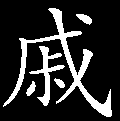
\includegraphics[width=3mm]{../Images/00005}  \kaishu 一物珍藏见至情,豪华每向闹中争。黛林宝薛传佳句,豪宴仙缘留趣名。为剪荷包绾两意,屈从优女结三生。可怜转眼皆虚话,云自飘飘月自明。}

{[}话说宝玉来{]}至院外\href{../Text/part0022_split_000.html\#lnkback_1_a}{\textsuperscript{①}},就有跟贾政的几个小厮上来拦腰抱住,都说:``今儿亏我们,老爷才喜欢,老太太打发人出来问了几遍,都亏我们回说喜欢;{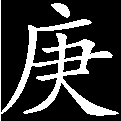
\includegraphics[width=3mm]{../Images/00004}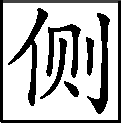
\includegraphics[width=3mm]{../Images/00011}\footnotesize \kaishu 下人口气毕肖。}不然,若老太太叫你进去,就不得展才了。人人都说,你才那些诗比世人的都强。今儿得了这样的彩头,该赏我们了。''宝玉笑道:``每人一吊钱。''众人道:``谁没见那一吊钱!{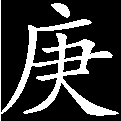
\includegraphics[width=3mm]{../Images/00004}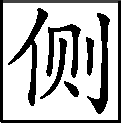
\includegraphics[width=3mm]{../Images/00011}\footnotesize \kaishu 钱亦有没用处。}把这荷包赏了罢。''说着,一个上来解荷包,那一个就解扇囊,不容分说,将宝玉所佩之物尽行解去。又道:``好生送上去罢。''一个抱了起来,几个围绕,送至贾母二门前。{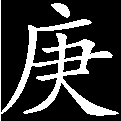
\includegraphics[width=3mm]{../Images/00004}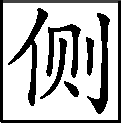
\includegraphics[width=3mm]{../Images/00011}\footnotesize \kaishu 好收煞。}那时贾母已命人看了几次。众奶娘丫鬟跟上来,见过贾母,知不曾难为着他,心中自是喜欢。

少时袭人倒了茶来,见身边佩物一件无存,{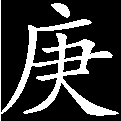
\includegraphics[width=3mm]{../Images/00004}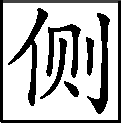
\includegraphics[width=3mm]{../Images/00011}\footnotesize \kaishu 袭人在玉兄一身,无时不照察到。}因笑道:``带的东西又是那起没脸的东西们解了去了。''林黛玉听说,走来瞧瞧,果然一件无存,因向宝玉道:``我给你的那个荷包也给他们了?{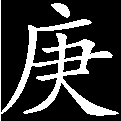
\includegraphics[width=3mm]{../Images/00004}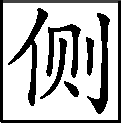
\includegraphics[width=3mm]{../Images/00011}\footnotesize \kaishu 又起楼阁。}你明儿再想我的东西,可不能够了!''说毕,赌气回房,将前日宝玉所烦他作的那个香袋儿------才做了一半------赌气拿过来就铰。宝玉见他生气,便知不妥,忙赶过来,早剪破了。宝玉已见过这香囊,虽尚未完,却十分精巧,费了许多工夫,今见无故剪了,却也可气。因忙把衣领解了,从里面红袄襟上将黛玉所给的那荷包解了下来,递与黛玉瞧道:``你瞧瞧,这是什么!我那一回把你的东西给人了?''林黛玉见他如此珍重,带在里面,{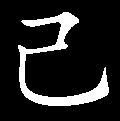
\includegraphics[width=3mm]{../Images/00003}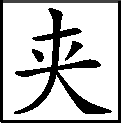
\includegraphics[width=3mm]{../Images/00012}\footnotesize \kaishu 按理论之,则是``天下本无事,庸人自扰之''。若以儿女子之情论之,则是必有之事,必有之理。又系今古小说中不能写到写得,谈情者亦不能说出讲出,情痴之至文也!}可知是怕人拿去之意,因此又自悔莽撞,未见皂白就剪了香袋,{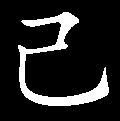
\includegraphics[width=3mm]{../Images/00003}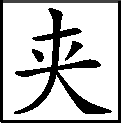
\includegraphics[width=3mm]{../Images/00012}\footnotesize \kaishu 情痴之至!若无此悔,便是一庸俗小性之女子矣。}因此又愧又气,低头一言不发。宝玉道:``你也不用剪,我知道你是懒待给我东西。我连这荷包奉还,何如?''说着,掷向他怀中便走。{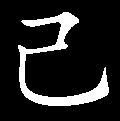
\includegraphics[width=3mm]{../Images/00003}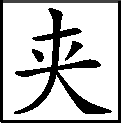
\includegraphics[width=3mm]{../Images/00012}\footnotesize \kaishu 这却难怪。}黛玉见如此,越发气起来,声咽气堵,又汪汪的滚下泪来,{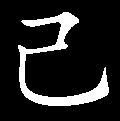
\includegraphics[width=3mm]{../Images/00003}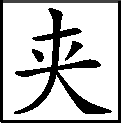
\includegraphics[width=3mm]{../Images/00012}\footnotesize \kaishu 怒之极,正是情之极。}拿起荷包来又剪。宝玉见他如此,忙回身抢住,笑道:``好妹妹,饶了他罢!''{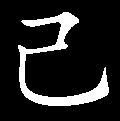
\includegraphics[width=3mm]{../Images/00003}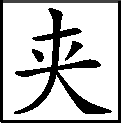
\includegraphics[width=3mm]{../Images/00012}\footnotesize \kaishu 这方是宝玉。}黛玉将剪子一摔,拭泪说道:``你不用同我好一阵歹一阵的,要恼,就撂开手。这当了什么!''说着,赌气上床,面向里倒下拭泪。禁不住宝玉上来``妹妹''长``妹妹''短赔不是。

前面贾母一片声找宝玉。众奶娘丫鬟们忙回说:``在林姑娘房里呢。''贾母听说道:``好,好,好!让他姊妹们一处顽顽罢。才他老子拘了他这半天,让他开心一会子罢。只别叫他们拌嘴,不许扭了他。''众人答应着。黛玉被宝玉缠不过,只得起来道:``你的意思不叫我安生,我就离了你。''说着往外就走。宝玉笑道:``你到那里,我跟到那里。''一面仍拿起荷包来带上。黛玉伸手抢道:``你说不要了,这会子又带上,我也替你怪臊的!''说着,``嗤''的一声笑了。宝玉道:``好妹妹,明儿另替我作个香袋儿罢。''黛玉道:``那也只瞧我高兴罢了。''一面说,一面二人出房,到王夫人上房中去了,{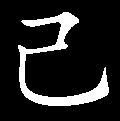
\includegraphics[width=3mm]{../Images/00003}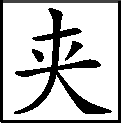
\includegraphics[width=3mm]{../Images/00012}\footnotesize \kaishu 一段点过近日二玉公案,断不可少。}可巧宝钗亦在那里。

此时王夫人那边热闹非常。{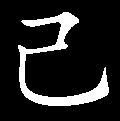
\includegraphics[width=3mm]{../Images/00003}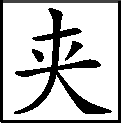
\includegraphics[width=3mm]{../Images/00012}\footnotesize \kaishu 四字特补近日千忙万冗,多少花团锦簇文字。}原来贾蔷已从姑苏采买了十二个女孩子,并聘了教习,以及行头等事来了。那时薛姨妈另迁于东北上一所幽静房舍居住,将梨香院早已腾挪出来,另行修理了,就令教习在此教演女戏。又另派家中旧有曾演学过歌唱的众女人们,如今皆已皤然老妪了,{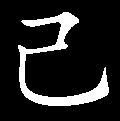
\includegraphics[width=3mm]{../Images/00003}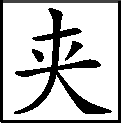
\includegraphics[width=3mm]{../Images/00012}\footnotesize \kaishu 又补出当日宁、荣在世之事,所谓此是末世之时也。}着他们带领管理。就令贾蔷总理其日用出入银钱等事,以及诸凡大小所需之物料账目。{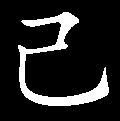
\includegraphics[width=3mm]{../Images/00003}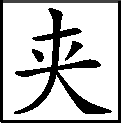
\includegraphics[width=3mm]{../Images/00012}\footnotesize \kaishu 补出女戏一段,又伏一案。}又有林之孝家的来回:``采访聘买得十个小尼姑、小道姑都有了,连新作的二十分道袍也有了。外有一个带发修行的,本是苏州人氏,祖上也是读书仕宦之家。因生了这位姑娘自小多病,买了许多替身儿皆不中用,足的这位姑娘亲自入了空门,方才好了,所以带发修行,今年才十八岁,法名妙玉。{{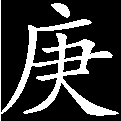
\includegraphics[width=3mm]{../Images/00004}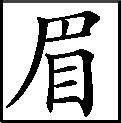
\includegraphics[width=3mm]{../Images/00010}\footnotesize \kaishu 妙玉世外人也,故笔笔带写,妙极妥极!畸笏。 }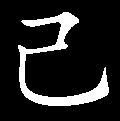
\includegraphics[width=3mm]{../Images/00003}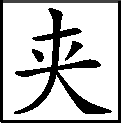
\includegraphics[width=3mm]{../Images/00012}\footnotesize \kaishu 妙卿出现。至此细数十二钗,以贾家四艳再加薛林二冠有六,添秦可卿有七,再凤有八,李纨有九,今又加妙玉,仅得十人矣。后有史湘云与熙凤之女巧姐儿者,共十二人,雪芹题曰``金陵十二钗'',盖本宗《红楼梦》十二曲之义。后宝琴、岫烟、李纹、李绮皆陪客也,《红楼梦》中所谓副十二钗是也。又有又副册三段词,乃晴雯、袭人、香菱三人而已,馀未多及,想为金钏、玉钏、鸳鸯、茜雪、平儿等人无疑矣。观者不待言可知,故不必多费笔墨。 {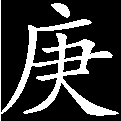
\includegraphics[width=3mm]{../Images/00004}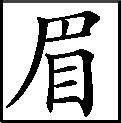
\includegraphics[width=3mm]{../Images/00010}\footnotesize \kaishu {(树处)}{[}副册{]}引十二钗总未的确,皆系漫拟也。至末回警幻情榜,方知正副、再副及三四副芳讳。壬午季春。畸笏。}}\href{../Text/part0022_split_000.html\#lnkback_2_a}{\textsuperscript{②}}如今父母俱已亡故,身边只有两个老嬷嬷,一个小丫头伏侍。文墨也极通,经文也不用学了,模样儿又极好。因听见长安都中有观音遗迹并贝叶遗文,去岁随了师父上来,{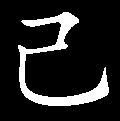
\includegraphics[width=3mm]{../Images/00003}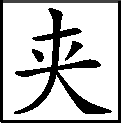
\includegraphics[width=3mm]{../Images/00012}\footnotesize \kaishu 因此方使妙卿入都。}现在西门外牟尼院住着。他师父极精演先天神数,于去冬圆寂了。妙玉本欲扶灵回乡的,他师父临寂遗言,说他`衣食起居不宜回乡,在此静居,后来自然有你的结果'。所以他竟未回。''王夫人不等回完,便说:``既这样,我们何不接了他来。''林之孝家的回道:``请他,他说:`侯门公府,必以贵势压人,我再不去的。'''{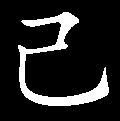
\includegraphics[width=3mm]{../Images/00003}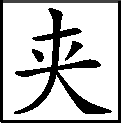
\includegraphics[width=3mm]{../Images/00012}\footnotesize \kaishu 补出妙卿身世不凡,心性高洁。}王夫人笑道:``他既是官宦小姐,自然骄傲些,就下个帖子请他何妨。''林之孝家的答应了出去,命书启相公写请帖去请妙玉。次日遣人备车轿去接等后话,暂且搁过,此时不能表白。{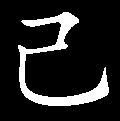
\includegraphics[width=3mm]{../Images/00003}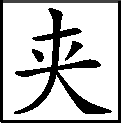
\includegraphics[width=3mm]{../Images/00012}\footnotesize \kaishu 补尼道一段,又伏一案。}\href{../Text/part0022_split_000.html\#lnkback_3_a}{\textsuperscript{③}}

当下又有人回,工程上等着糊东西的纱绫,请凤姐去开楼拣纱绫;又有人来回,请凤姐开库,收金银器皿。连王夫人并上房丫鬟等众,皆一时不得闲的。宝钗便说:``咱们别在这里碍手碍脚,找探丫头去。''说着,同宝玉黛玉往迎春等房中来闲顽,无话。

王夫人等日日忙乱,直到十月将尽,幸皆全备:各处监管都交清账目;各处古董文玩,皆已陈设齐备;采办鸟雀的,自仙鹤、孔雀以及鹿、兔、鸡、鹅等类,悉已买全,交于园中各处像景饲养;贾蔷那边也演出二十出杂戏来;小尼姑、道姑也都学会了念几卷经咒。贾政方略心意宽畅,{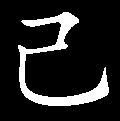
\includegraphics[width=3mm]{../Images/00003}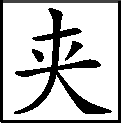
\includegraphics[width=3mm]{../Images/00012}\footnotesize \kaishu 好极!可见智者居心无一时弛怠!}又请贾母等进园,色色斟酌,点缀妥当,再无一些遗漏不当之处了。于是贾政方择日题本。{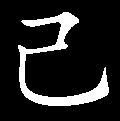
\includegraphics[width=3mm]{../Images/00003}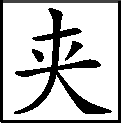
\includegraphics[width=3mm]{../Images/00012}\footnotesize \kaishu 至此方完大观园工程公案。观者则为大观园费尽精神,余则为若许笔墨,却只因一个葬花冢。}本上之日,奉朱批准奏:次年正月十五日上元之日,恩准贵妃省亲。贾府领了此恩旨,益发昼夜不闲,年也不曾好生过的。{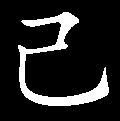
\includegraphics[width=3mm]{../Images/00003}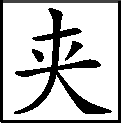
\includegraphics[width=3mm]{../Images/00012}\footnotesize \kaishu 一语带过。是以``岁首祭宗祠,元宵开家宴''一回留在后文细写。}

展眼元宵在迩,自正月初八日,就有太监出来先看方向:何处更衣,何处燕坐,何处受礼,何处开宴,何处退息。又有巡察地方总理关防太监等,带了许多小太监出来,各处关防,挡围幕,指示贾宅人员何处退,何处跪,何处进膳,何处启事,种种仪注不一。外面又有工部官员并五城兵备道打扫街道,撵逐闲人。贾赦等督率匠人扎花灯烟火之类,至十四日,俱已停妥。这一夜,上下通不曾睡。

至十五日五鼓,自贾母等有爵者,俱各按品服大妆。园内各处,帐舞蟠龙,帘飞彩凤,金银焕彩,珠宝争辉,{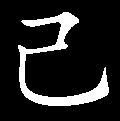
\includegraphics[width=3mm]{../Images/00003}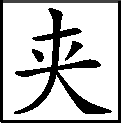
\includegraphics[width=3mm]{../Images/00012}\footnotesize \kaishu 是元宵之夕,不写灯月而灯光月色满纸矣。}鼎焚百合之香,瓶插长春之蕊,{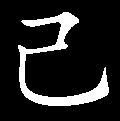
\includegraphics[width=3mm]{../Images/00003}\includegraphics[width=3mm]{../Images/00012}\footnotesize \kaishu 抵一篇大赋。}静悄无人咳嗽。{\includegraphics[width=3mm]{../Images/00003}\includegraphics[width=3mm]{../Images/00012}\footnotesize \kaishu 有此句方足。}贾赦等在西街门外,贾母等在荣府大门外。街头巷口,俱系围幕挡严。正等的不耐烦,忽一太监坐大马而来,{\includegraphics[width=3mm]{../Images/00003}\includegraphics[width=3mm]{../Images/00012}\footnotesize \kaishu 有是礼。}贾母忙接入,问其消息。太监道:``早多着呢!未初刻用过晚膳,未正二刻还到宝灵宫拜佛,{\includegraphics[width=3mm]{../Images/00003}\includegraphics[width=3mm]{../Images/00012}\footnotesize \kaishu 暗贴王夫人,细。}酉初刻进大明宫领宴看灯方请旨,只怕戌初才起身呢。''凤姐听了道:{\includegraphics[width=3mm]{../Images/00004}\includegraphics[width=3mm]{../Images/00011}\footnotesize \kaishu 自然当家人先说话。}``既是这么着,老太太、太太且请回房,等是时候再来也不迟。''于是贾母等暂且自便,园中悉赖凤姐照理。又命执事人带领太监们去吃酒饭。

一时传人一担一担的挑进蜡烛来,各处点灯。方点完时,忽听外边马跑之声。{\includegraphics[width=3mm]{../Images/00003}\includegraphics[width=3mm]{../Images/00012}\footnotesize \kaishu 静极故闻之。细极。}一时,有十来个太监都喘吁吁跑来拍手儿。{\includegraphics[width=3mm]{../Images/00003}\includegraphics[width=3mm]{../Images/00012}\footnotesize \kaishu 画出内家风范。《石头记》最难之处,别书中摸不着。}这些太监会意,{\includegraphics[width=3mm]{../Images/00004}\includegraphics[width=3mm]{../Images/00011}\footnotesize \kaishu 难得他{[}写{]}的出,是经过之人也。}都知道是``来了,来了'',各按方向站住。贾赦领合族子侄在西街门外,贾母领合族女眷在大门外迎接。半日静悄悄的。忽见一对红衣太监骑马缓缓的走来,{\includegraphics[width=3mm]{../Images/00003}\includegraphics[width=3mm]{../Images/00012}\footnotesize \kaishu 形容毕肖。}至西街门下了马,将马赶出围幕之外,便垂手面西站住。{\includegraphics[width=3mm]{../Images/00003}\includegraphics[width=3mm]{../Images/00012}\footnotesize \kaishu 形容毕肖。}半日又是一对,亦是如此。少时便来了十来对,方闻得隐隐细乐之声。一对对龙旌凤翣,雉羽夔头,又有销金提炉焚着御香;然后一把曲柄七凤黄金伞过来,便是冠袍带履。又有随事太监捧着香珠、绣帕、漱盂、拂尘等类。一队队过完,后面方是八个太监抬着一顶金顶金黄绣凤版舆,缓缓行来。贾母等连忙路旁跪下。{\includegraphics[width=3mm]{../Images/00004}\includegraphics[width=3mm]{../Images/00011}\footnotesize \kaishu 一丝不乱。}早飞跑过几个太监来,扶起贾母、邢夫人、王夫人来。那版舆抬进大门、入仪门往东,去到一所院落门前,有执拂太监跪请下舆更衣。于是抬舆入门,太监等散去,只有昭容、彩嫔等引领元春下舆。只见院内各色花灯熌灼,{\includegraphics[width=3mm]{../Images/00004}\includegraphics[width=3mm]{../Images/00011}\footnotesize \kaishu 元春目中。}皆系纱绫扎成,精致非常。上面有一匾灯,写着``体仁沐德''四字。元春入室,更衣毕复出,上舆进园。只见园中香烟缭绕,花彩缤纷,处处灯光相映,时时细乐声喧,说不尽这太平景象、富贵风流。此时自己回想当初在大荒山中,青埂峰下,那等凄凉寂寞;若不亏癞僧、跛道二人携来到此,又安能得见这般世面。本欲作一篇《灯月赋》、《省亲颂》,以志今日之事,但又恐入了别书的俗套。按此时之景,即作一赋一赞,也不能形容得尽其妙;即不作赋赞,其豪华富丽,观者诸公亦可想而知矣。所以倒是省了这工夫纸墨,且说正紧的为是。{\includegraphics[width=3mm]{../Images/00003}\includegraphics[width=3mm]{../Images/00012}\footnotesize \kaishu 自``此时''以下皆石头之语,真是千奇百怪之文。 {\includegraphics[width=3mm]{../Images/00004}\includegraphics[width=3mm]{../Images/00010}\footnotesize \kaishu 如此繁华盛极、花团锦簇之文,忽用石兄自语截住,是何笔力!令人安得不拍案叫绝。试阅历来诸小说中有如此章法乎?}}

且说贾妃在轿内看此园内外如此豪华,因默默叹息奢华过费。忽又见执拂太监跪请登舟。贾妃乃下舆。只见清流一带,势如游龙,两边石栏上,皆系水晶玻璃各色风灯,点的如银光雪浪;上面柳杏诸树虽无花叶,然皆用通草绸绫纸绢依势作成,粘于枝上的,每一株悬灯数盏;更兼池中荷荇凫鹭之属,亦皆系螺蚌羽毛之类作就的。诸灯上下争辉,真系玻璃世界,珠宝乾坤。船上亦系各种精致盆景诸灯,珠帘绣幕,桂楫兰桡,自不必说。已而入一石港,港上一面匾灯,明现着``蓼汀花溆''四字。按此四字,并``有凤来仪''等处,皆系上回贾政偶然一试宝玉之课艺才情耳,何今日认真用此匾联?况贾政世代诗书,来往诸客屏侍坐陪者,悉皆才技之流,岂无一名手题撰,竟用小儿一戏之辞苟且搪塞?{\includegraphics[width=3mm]{../Images/00004}\includegraphics[width=3mm]{../Images/00010}\footnotesize \kaishu 驳得好!}真似暴发新荣之家,滥使银钱,一味抹油涂朱,毕则大书``前门绿柳垂金锁,后户青山列锦屏''之类,则以为大雅可观,岂《石头记》中通部所表之宁荣贾府所为哉!据此论之,竟大相矛盾了。诸公不知,待蠢物{\includegraphics[width=3mm]{../Images/00003}\includegraphics[width=3mm]{../Images/00012}\footnotesize \kaishu 石兄自谦,妙!可代答云``岂敢!''}将原委说明,大家方知。{\includegraphics[width=3mm]{../Images/00004}\includegraphics[width=3mm]{../Images/00010}\footnotesize \kaishu 《石头记》惯用特犯不犯之笔,读之真令人惊心骇目。}

当日这贾妃未入宫时,自幼亦系贾母教养。后来添了宝玉,贾妃乃长姊,宝玉为弱弟,贾妃之心上念母年将迈,始得此弟,是以怜爱宝玉,与诸弟待之不同。且同随贾母,刻未暂离。那宝玉未入学堂之先,三四岁时,已得贾妃手引口传,教授了几本书、数千字在腹内了。{\includegraphics[width=3mm]{../Images/00004}\includegraphics[width=3mm]{../Images/00011}\footnotesize \kaishu 批书人领过此教,故批至此竟放声大哭,俺先姊仙逝太早,不然余何得为废人耶?}其名分虽系姊弟,其情状有如母子。自入宫后,时时带信出来与父母说:``千万好生扶养,不严不能成器,过严恐生不虞,且致父母之忧。''眷念切爱之心,刻未能忘。前日贾政闻塾师背后赞宝玉偏才尽有,贾政未信,适巧遇园已落成,令其题撰,聊一试其情思之清浊。其所拟之匾联虽非妙句,在幼童为之,亦或可取。即另使名公大笔为之,固不费难,然想来倒不如这本家风味有趣。{\includegraphics[width=3mm]{../Images/00004}\includegraphics[width=3mm]{../Images/00011}\footnotesize \kaishu 转得好。}更使贾妃见之,知系其爱弟所为,亦或不负其素日切望之意。{\includegraphics[width=3mm]{../Images/00003}\includegraphics[width=3mm]{../Images/00012}\footnotesize \kaishu 一驳一解,跌宕摇曳之至,且写得父母兄弟体贴恋爱之情,淋漓痛切,真是天伦至情。 {\includegraphics[width=3mm]{../Images/00004}\includegraphics[width=3mm]{../Images/00011}\footnotesize \kaishu 有是论。}}因有这段原委,故此竟用了宝玉所题之联额。那日虽未曾题完,后来亦曾补拟。{\includegraphics[width=3mm]{../Images/00003}\includegraphics[width=3mm]{../Images/00012}\footnotesize \kaishu 一句补前文之不暇,启后文之苗裔。至后文凹晶馆黛玉口中又一补,所谓``一击空谷,八方皆应''。}

闲文少叙,且说贾妃看了四字,笑道:``\,`花溆'二字便妥,何必`蓼汀'?''侍座太监听了,忙下小舟登岸,飞传与贾政。贾政听了,即忙移换。{\includegraphics[width=3mm]{../Images/00003}\includegraphics[width=3mm]{../Images/00012}\footnotesize \kaishu 换的周到可悦。}一时,舟临内岸,复弃舟上舆,便见琳宫绰约,桂殿巍峨。石牌坊上明显``天仙宝境''四字,{\includegraphics[width=3mm]{../Images/00003}\includegraphics[width=3mm]{../Images/00012}\footnotesize \kaishu 不得不用俗。}贾妃忙命换``省亲别墅''四字。{\includegraphics[width=3mm]{../Images/00003}\includegraphics[width=3mm]{../Images/00012}\footnotesize \kaishu 妙!是特留此四字与彼自命。}于是进入行宫。但见庭燎烧空,{\includegraphics[width=3mm]{../Images/00003}\includegraphics[width=3mm]{../Images/00012}\footnotesize \kaishu ``庭燎''最恰。}香屑布地,火树琪花,金窗玉槛。说不尽帘卷虾须,毯铺鱼獭,鼎飘麝脑之香,屏列雉尾之扇。真是:

金门玉户神仙府,桂殿兰宫妃子家。

贾妃乃问:``此殿何无匾额?''随侍太监跪启曰:``此系正殿,外臣未敢擅拟。''贾妃点头不语。礼仪太监跪请升座受礼,两陛乐起。礼仪太监二人引贾赦、贾政等于月台下排班,殿上昭容传谕曰:``免。''太监引贾赦等退出。又有太监引荣国太君及女眷等自东阶升月台上排班,{\includegraphics[width=3mm]{../Images/00003}\includegraphics[width=3mm]{../Images/00012}\footnotesize \kaishu 一丝不乱,精致大方。有如欧阳公九九。}昭容再谕曰:``免。''于是引退。

茶已三献,贾妃降座,乐止。退入侧殿更衣,方备省亲车驾出园。至贾母正室,欲行家礼,贾母等俱跪止不迭。贾妃满眼垂泪,方彼此上前厮见,一手搀贾母,一手搀王夫人,三个人满心里皆有许多话,只是俱说不出,只管呜咽对泣。{\includegraphics[width=3mm]{../Images/00003}\includegraphics[width=3mm]{../Images/00012}\footnotesize \kaishu 《石头记》得力擅长,全是此等地方。 {\includegraphics[width=3mm]{../Images/00004}\includegraphics[width=3mm]{../Images/00010}\footnotesize \kaishu 非经历过如何写得出!壬午春。}}邢夫人、李纨、王熙凤、迎、探、惜三姊妹等,俱在旁围绕,垂泪无言。半日,贾妃方忍悲强笑,安慰贾母、王夫人道:``当日既送我到那不得见人的去处,好容易今日回家娘儿们一会,不说说笑笑,反倒哭起来。一会子我去了,又不知多早晚才来!''说到这句,不禁又哽咽起来。{\includegraphics[width=3mm]{../Images/00003}\includegraphics[width=3mm]{../Images/00012}\footnotesize \kaishu 追魂摄魄。《石头记》传神摹影,全在此等地方,他书中不得有此见识。}邢夫人等忙上来解劝。{\includegraphics[width=3mm]{../Images/00003}\includegraphics[width=3mm]{../Images/00012}\footnotesize \kaishu 说完不可,不先说不可,说之不痛不可,最难说者是此时贾妃口中之语。只如此一说,方千贴万妥,一字不可更改,一字不可增减,入情入神之至!}贾母等让贾妃归座,又逐次一一见过,又不免哭泣一番。然后东西两府掌家执事人丁等在厅外行礼,及两府掌家执事媳妇领丫鬟等行礼毕。贾妃因问:``薛姨妈、宝钗、黛玉因何不见?''{\includegraphics[width=3mm]{../Images/00009}\includegraphics[width=3mm]{../Images/00012}\footnotesize \kaishu 谅前信息皆知,故有此问。}王夫人启曰:``外眷无职,未敢擅入。''{\includegraphics[width=3mm]{../Images/00003}\includegraphics[width=3mm]{../Images/00012}\footnotesize \kaishu 所谓诗书世家,守礼如此。偏是暴发,骄妄自大。}贾妃听了,忙命快请。{\includegraphics[width=3mm]{../Images/00003}\includegraphics[width=3mm]{../Images/00012}\footnotesize \kaishu 又谦之如此,真是世界好人物。}一时薛姨妈等进来,欲行国礼,亦命免过,上前各叙阔别寒温。又有贾妃原带进宫去的丫鬟抱琴等{\includegraphics[width=3mm]{../Images/00003}\includegraphics[width=3mm]{../Images/00012}\footnotesize \kaishu 前所谓贾家四钗之鬟,暗以琴棋书画排行,至此始全。}上来叩见,贾母等连忙扶起,命人别室款待。执事太监及彩嫔、昭容各侍从人等,宁国府及贾赦那宅两处自有人款待,只留三四个小太监答应。母女姊妹深叙些离别情景,{\includegraphics[width=3mm]{../Images/00003}\includegraphics[width=3mm]{../Images/00012}\footnotesize \kaishu ``深''字妙!}及家务私情。

又有贾政至帘外问安,贾妃垂帘行参等事。又隔帘含泪谓其父曰:``田舍之家,虽齑盐布帛,终能聚天伦之乐;今虽富贵已极,骨肉各方,然终无意趣!''贾政亦含泪启道:``臣草莽寒门,鸠群鸦属之中,岂意得征凤鸾之瑞。{\includegraphics[width=3mm]{../Images/00004}\includegraphics[width=3mm]{../Images/00011}\footnotesize \kaishu 此语犹在耳。}今贵人上锡天恩,下昭祖德,此皆山川日月之精奇、祖宗之远德钟于一人,幸及政夫妇。且今上启天地生物之大德,垂古今未有之旷恩,虽肝脑涂地,臣子岂能得报于万一!惟朝乾夕惕,忠于厥职外,愿我君万寿千秋,乃天下苍生之同幸也。贵妃切勿以政夫妇残犁为念,懑愤金怀,更祈自加珍爱。惟业业兢兢,勤慎恭肃以侍上,庶不负上体贴眷爱如此之隆恩也。''贾妃亦嘱``只以国事为重,暇时保养,切勿记念''等语。贾政又启:``园中所有亭台轩馆,皆系宝玉所题。如果有一二稍可寓目者,请别赐名为幸。''元妃听了宝玉能题,便含笑说:``果进益了。''贾政退出。贾妃见宝、林二人亦发比别姊妹不同,真是姣花软玉一般。因问:``宝玉为何不进见?''{\includegraphics[width=3mm]{../Images/00003}\includegraphics[width=3mm]{../Images/00012}\footnotesize \kaishu 至此方出宝玉。}贾母乃启:``无谕,外男不敢擅入。''元妃命快引进来。小太监出去引宝玉进来,先行国礼毕,元妃命他进前,携手揽于怀内,又抚其头颈,{\includegraphics[width=3mm]{../Images/00004}\includegraphics[width=3mm]{../Images/00011}\footnotesize \kaishu 作书人将批书人哭坏了。}笑道:``比先竟长了好些\ldots{}\ldots{}''一语未终,泪如雨下。{\includegraphics[width=3mm]{../Images/00003}\includegraphics[width=3mm]{../Images/00012}\footnotesize \kaishu 只此一句,便补足前面许多文字。}

尤氏、凤姐等上来启道:``筵宴齐备,请贵妃游幸。''元妃等起身,命宝玉导引,遂同诸人步至园门前。早见灯光火树之中,诸般罗列非常。进园来先从``有凤来仪''、``红香绿玉''、``杏帘在望''、``蘅芷清芬''等处,登楼步阁,涉水缘山,百般眺览徘徊。一处处铺陈不一,一桩桩点缀新奇。贾妃极加奖赞,又劝:``以后不可太奢,此皆过分之极。''已而至正殿,谕免礼归座,大开筵宴。贾母等在下相陪,尤氏、李纨、凤姐等亲捧羹把盏。

元妃乃命传笔砚伺候,亲搦湘管,择其几处最喜者赐名。按其书云:

``顾恩思义''{匾额}

天地启宏慈,赤子苍头同感戴;

古今垂旷典,九州万国被恩荣。{此一匾一联书于正殿。{\includegraphics[width=3mm]{../Images/00003}\includegraphics[width=3mm]{../Images/00012}\footnotesize \kaishu 是贵妃口气。}}

``大观园''{园之名}

``有凤来仪''{赐名曰``潇湘馆''。}

``红香绿玉''改作``怡红快绿''。{即名曰``怡红院''。}

``蘅芷清芬''{赐名曰``蘅芜苑''。}

``杏帘在望''{赐名曰``浣葛山庄''。}

正楼曰``大观楼'',东面飞楼曰``缀锦阁'',西面斜楼曰``含芳阁'';更有``蓼风轩''、``藕香榭''、{\includegraphics[width=3mm]{../Images/00003}\includegraphics[width=3mm]{../Images/00012}\footnotesize \kaishu 雅而新。}``紫菱洲''、``荇叶渚''等名;又有四字的匾额十数个,诸如``梨花春雨''、``桐剪秋风''、``荻芦夜雪''等名,此时悉难全记。{\includegraphics[width=3mm]{../Images/00003}\includegraphics[width=3mm]{../Images/00012}\footnotesize \kaishu 故意留下秋爽斋、凸碧山堂、凹晶溪馆、暖香坞等处为后文另换眼目之地步。}又命旧有匾联俱不必摘去。于是先题一绝云:

衔山抱水建来精,多少工夫筑始成。

天上人间诸景备,芳园应锡大观名。{\includegraphics[width=3mm]{../Images/00003}\includegraphics[width=3mm]{../Images/00012}\footnotesize \kaishu 诗却平平,盖彼不长于此也,故只如此。}

写毕,向诸姐妹笑道:``我素乏捷才,且不长于吟咏,妹辈素所深知。今夜聊以塞责,不负斯景而已。异日少暇,必补撰《大观园记》并《省亲颂》等文,以记今日之事。妹辈亦各题一匾一诗,随才之长短,亦暂吟成,不可因我微才所缚。且喜宝玉竟知题咏,是我意外之想。此中`潇湘馆'、`蘅芜苑'二处,我所极爱,次之`怡红院'、`浣葛山庄',此四大处,必得别有章句题咏方妙。前所题之联虽佳,如今再各赋五言律一首,使我当面试过,方不负我自幼教授之苦心。''宝玉只得答应了,下来自去构思。

迎、探、惜三人之中,要算探春又出于姊妹之上,然自忖亦难与薛林争衡,{\includegraphics[width=3mm]{../Images/00003}\includegraphics[width=3mm]{../Images/00012}\footnotesize \kaishu 只一语,便写出宝黛二人,又写出探卿知己知彼,伏下后文多少地步。}只得勉强随众塞责而已。李纨也勉强凑成一律。{\includegraphics[width=3mm]{../Images/00003}\includegraphics[width=3mm]{../Images/00012}\footnotesize \kaishu 不表薛、林可知。}贾妃先挨次看姊妹们的,写道是:

旷性怡情 {匾额} 迎 春

园成景备特精奇,奉命羞题额旷怡。

谁信世间有此境,游来宁不畅神思?

万象争辉 {匾额} 探 春

名园筑出势巍巍,奉命何惭学浅微。

精妙一时言不出,果然万物生光辉。

文章造化 {匾额} 惜 春

山水横拖千里外,楼台高起五云中。

园修日月光辉里,景夺文章造化功。{\includegraphics[width=3mm]{../Images/00003}\includegraphics[width=3mm]{../Images/00012}\footnotesize \kaishu 更牵强。三首之中还算探卿略有作意,故后文写出许多意外妙文。}

文采风流 {匾额} 李 纨

秀水明山抱复回,风流文采胜蓬莱。{\includegraphics[width=3mm]{../Images/00003}\includegraphics[width=3mm]{../Images/00012}\footnotesize \kaishu 起好!}

绿裁歌扇迷芳草,红衬湘裙舞落梅。{\includegraphics[width=3mm]{../Images/00003}\includegraphics[width=3mm]{../Images/00012}\footnotesize \kaishu 凑成。}

珠玉自应传盛世,神仙何幸下瑶台。

名园一自邀游赏,未许凡人到此来。{{\includegraphics[width=3mm]{../Images/00003}\includegraphics[width=3mm]{../Images/00012}\footnotesize \kaishu 此四诗列于前,正为}滃{托下韵也。}}

凝晖钟瑞
{匾额{\includegraphics[width=3mm]{../Images/00003}\includegraphics[width=3mm]{../Images/00012}\footnotesize \kaishu 便有含蓄。}} 薛宝钗

芳园筑向帝城西,华日祥云笼罩奇。

高柳喜迁莺出谷,修篁时待凤来仪。{\includegraphics[width=3mm]{../Images/00003}\includegraphics[width=3mm]{../Images/00012}\footnotesize \kaishu 恰极!}

文风已着宸游夕,孝化应隆归省时。

睿藻仙才盈彩笔,自惭何敢再为辞?{\includegraphics[width=3mm]{../Images/00003}\includegraphics[width=3mm]{../Images/00012}\footnotesize \kaishu 好诗!此不过颂圣应制耳,犹未见长,以后渐知。}

世外仙源
{匾额{\includegraphics[width=3mm]{../Images/00003}\includegraphics[width=3mm]{../Images/00012}\footnotesize \kaishu 落想便不与人同。}} 林黛玉

名园筑何处,仙境别红尘。

借得山川秀,添来景物新。{\includegraphics[width=3mm]{../Images/00003}\includegraphics[width=3mm]{../Images/00012}\footnotesize \kaishu 所谓``信手拈来无不是''。◇阿颦自是一种心思。}

香融金谷酒,花媚玉堂人。

何幸邀恩宠,宫车过往频?{\includegraphics[width=3mm]{../Images/00003}\includegraphics[width=3mm]{../Images/00012}\footnotesize \kaishu 末二首是应制诗。◇余谓宝、林此作未见长,何也?盖后文别有惊人之句也。在宝卿有生不屑为此,在黛卿实不足一为。}

贾妃看毕,称赏一番,又笑道:``终是薛林二妹之作与众不同,非愚姊妹可同列者。''原来林黛玉安心今夜大展奇才,将众人压倒,{\includegraphics[width=3mm]{../Images/00003}\includegraphics[width=3mm]{../Images/00012}\footnotesize \kaishu 这却何必,然尤物方如此。}不想贾妃只命一匾一咏,倒不好违谕多作,只胡乱作一首五言律应景罢了。{\includegraphics[width=3mm]{../Images/00003}\includegraphics[width=3mm]{../Images/00012}\footnotesize \kaishu 请看前诗,却云是胡乱应景。}

彼时宝玉尚未作完,只刚做了``潇湘馆''与``蘅芜苑''二首,正作``怡红院''一首,起草内有``绿玉春犹卷''一句。宝钗转眼瞥见,便趁众人不理论,急忙回身悄推他道:``他{\includegraphics[width=3mm]{../Images/00003}\includegraphics[width=3mm]{../Images/00012}\footnotesize \kaishu 此``他''字指贾妃。 {\includegraphics[width=3mm]{../Images/00004}\includegraphics[width=3mm]{../Images/00010}\footnotesize \kaishu 这样章法,又是不曾见过的。}}因不喜`红香绿玉'四字,改了`怡红快绿';你这会子偏用`绿玉'二字,岂不是有意和他争驰了?况且蕉叶之说也颇多,再想一个字改了罢。''宝玉见宝钗如此说,便拭汗道:{\includegraphics[width=3mm]{../Images/00003}\includegraphics[width=3mm]{../Images/00012}\footnotesize \kaishu 想见其构思之苦,方是至情。最厌近之小说中满纸``神童''、``天分''等语。}``我这会子总想不起什么典故出处来。''宝钗笑道:``你只把`绿玉'的`玉'字改作`蜡'字就是了。''宝玉道:```绿蜡'{\includegraphics[width=3mm]{../Images/00004}\includegraphics[width=3mm]{../Images/00011}\footnotesize \kaishu 好极!}可有出处?''宝钗见问,悄悄的咂嘴点头{\includegraphics[width=3mm]{../Images/00004}\includegraphics[width=3mm]{../Images/00011}\footnotesize \kaishu 媚极!韵极!}笑道:``亏你今夜不过如此,将来金殿对策,你大约连`赵钱孙李'都忘了呢!{\includegraphics[width=3mm]{../Images/00003}\includegraphics[width=3mm]{../Images/00012}\footnotesize \kaishu 有得宝卿奚落。但{(就)}{[}孰{]}谓宝卿无情?只是较阿颦施之特正耳。}唐钱珝咏芭蕉诗头一句`冷烛无烟绿蜡干',你都忘了不成?''{\includegraphics[width=3mm]{../Images/00003}\includegraphics[width=3mm]{../Images/00012}\footnotesize \kaishu 此等处便用硬证实处,最是大力量,但不知是何心思,是从何落想,穿插到如此玲珑锦绣地步。 {\includegraphics[width=3mm]{../Images/00004}\includegraphics[width=3mm]{../Images/00010}\footnotesize \kaishu 如此穿插,安得不令人拍案叫绝!壬午季春。 }\includegraphics[width=3mm]{../Images/00009}\includegraphics[width=3mm]{../Images/00012}\footnotesize \kaishu 乃翁前何多敏捷,今见乃姐何反迟钝,未免怯才,拘紧人所必有之耳。}宝玉听了,不觉洞开心臆,笑道:``该死,该死!现成眼前之物偏倒想不起来了,真可谓`一字师'了。从此后我只叫你师父,再不叫姐姐了。''宝钗亦悄悄的笑道:``还不快作上去,只管姐姐妹妹的。谁是你姐姐?那上头穿黄袍的才是你姐姐,你又认我这姐姐来了。''一面说笑,因说笑又怕他耽延工夫,遂抽身走开了。{\includegraphics[width=3mm]{../Images/00003}\includegraphics[width=3mm]{../Images/00012}\footnotesize \kaishu 一段忙中闲文,已是好看之极,出人意外。}宝玉只得续成,共有了三首。

此时林黛玉未得展其抱负,自是不快。因见宝玉独作四律,大费神思,何不代他作两首,也省他些精神不到之处。{\includegraphics[width=3mm]{../Images/00003}\includegraphics[width=3mm]{../Images/00012}\footnotesize \kaishu 写黛卿之情思,待宝玉却又如此,是与前文特犯不犯之处。 {\includegraphics[width=3mm]{../Images/00004}\includegraphics[width=3mm]{../Images/00010}\footnotesize \kaishu 偏又写一样,是何心意构思而得?畸笏。}}想着,便也走至宝玉案旁,悄问:``可都有了?''宝玉道:``才有了三首,只少`杏帘在望'一首了。''黛玉道:``既如此,你只抄录前三首罢。赶你写完那三首,我也替你作出这首了。''说毕,低头一想,早已吟成一律,{\includegraphics[width=3mm]{../Images/00003}\includegraphics[width=3mm]{../Images/00012}\footnotesize \kaishu 瞧他写阿颦,只如此便妙极。}便写在纸条上,搓成个团子,掷在他跟前。{{\includegraphics[width=3mm]{../Images/00004}\includegraphics[width=3mm]{../Images/00010}\footnotesize \kaishu 纸条送递系应{[}试{]}童生秘诀,黛卿自何处学得?一笑。丁亥春。 }\includegraphics[width=3mm]{../Images/00009}\includegraphics[width=3mm]{../Images/00012}\footnotesize \kaishu 姐姐做试官尚用枪手,难怪世间之代倩多耳。}宝玉打开一看,只觉此首比自己所作的三首高过十倍,真是喜出望外,{\includegraphics[width=3mm]{../Images/00003}\includegraphics[width=3mm]{../Images/00012}\footnotesize \kaishu 这等文字,亦是观书者望外之想。}遂忙恭楷呈上。贾妃看道:

有凤来仪 臣宝玉谨题

秀玉初成实,堪宜待凤凰。{\includegraphics[width=3mm]{../Images/00003}\includegraphics[width=3mm]{../Images/00012}\footnotesize \kaishu 起便拿得住。}

竿竿青欲滴,个个绿生凉。

迸砌防阶水,穿帘碍鼎香。{\includegraphics[width=3mm]{../Images/00003}\includegraphics[width=3mm]{../Images/00012}\footnotesize \kaishu 妙句!古云:``竹密何妨水过'',今偏翻案。}

莫摇清碎影,好梦昼初长。

蘅芷清芬

蘅芜满净苑,萝薜助芬芳。{\includegraphics[width=3mm]{../Images/00003}\includegraphics[width=3mm]{../Images/00012}\footnotesize \kaishu ``助''字妙!通部书所以皆善炼字。}

软衬三春草,柔拖一缕香。{\includegraphics[width=3mm]{../Images/00003}\includegraphics[width=3mm]{../Images/00012}\footnotesize \kaishu 刻画入妙。}

轻烟迷曲径,冷翠滴回廊。{\includegraphics[width=3mm]{../Images/00003}\includegraphics[width=3mm]{../Images/00012}\footnotesize \kaishu 甜脆满颊。}

谁谓池塘曲,谢家幽梦长。

怡红快绿

深庭长日静,两两出婵娟。{\includegraphics[width=3mm]{../Images/00003}\includegraphics[width=3mm]{../Images/00012}\footnotesize \kaishu 双起双敲,读此首始信前云``有蕉无棠不可,有棠无蕉更不可''等批,非泛泛妄批驳他人,到自己身上则无能为之论也。}

绿蜡{\includegraphics[width=3mm]{../Images/00003}\includegraphics[width=3mm]{../Images/00012}\footnotesize \kaishu 本是``玉''字,此遵宝卿改,似较``玉''字佳。}春犹卷,{\includegraphics[width=3mm]{../Images/00003}\includegraphics[width=3mm]{../Images/00012}\footnotesize \kaishu 是蕉。}红妆夜未眠。{\includegraphics[width=3mm]{../Images/00003}\includegraphics[width=3mm]{../Images/00012}\footnotesize \kaishu 是海棠。}

凭栏垂绛袖,{\includegraphics[width=3mm]{../Images/00003}\includegraphics[width=3mm]{../Images/00012}\footnotesize \kaishu 是海棠之情。}倚石护青烟。{\includegraphics[width=3mm]{../Images/00003}\includegraphics[width=3mm]{../Images/00012}\footnotesize \kaishu 是芭蕉之神。何得如此工恰自然?真是好诗,却是好书。}

对立东风里,{\includegraphics[width=3mm]{../Images/00003}\includegraphics[width=3mm]{../Images/00012}\footnotesize \kaishu 双收。}主人应解怜。{\includegraphics[width=3mm]{../Images/00003}\includegraphics[width=3mm]{../Images/00012}\footnotesize \kaishu 归到主人方不落空。◇王梅隐云:``咏物体又难双承双落,一味双拿则不免牵强。''此首可谓诗题两称,极工、极切、极流{(离)}{[}丽{]}妩媚。}

杏帘在望

杏帘招客饮,在望有山庄。{\includegraphics[width=3mm]{../Images/00003}\includegraphics[width=3mm]{../Images/00012}\footnotesize \kaishu 分题作一气呵成,格调熟练,自是阿颦口气。}

菱荇鹅儿水,桑榆燕子梁。{\includegraphics[width=3mm]{../Images/00003}\includegraphics[width=3mm]{../Images/00012}\footnotesize \kaishu 阿颦之心臆才情原与人别,亦不是从读书中得来。}

一畦春韭绿,十里稻花香。

盛世无饥馁,何须耕织忙。{\includegraphics[width=3mm]{../Images/00003}\includegraphics[width=3mm]{../Images/00012}\footnotesize \kaishu 以幻入幻,顺水推舟,且不失应制,所以称阿颦。}

贾妃看毕,喜之不尽,说:``果然进益了!''又指``杏帘''一首为前三首之冠。遂将``浣葛山庄''改为``稻香村''。{\includegraphics[width=3mm]{../Images/00003}\includegraphics[width=3mm]{../Images/00012}\footnotesize \kaishu 如此服善,妙! {\includegraphics[width=3mm]{../Images/00004}\includegraphics[width=3mm]{../Images/00010}\footnotesize \kaishu 仍用玉兄前拟``稻香村'',却如此幻笔幻体,文章之格式,至矣尽矣!壬午春。}}又命探春另以彩笺誊录出方才一共十数首诗,出令太监传与外厢。贾政等看了,都称颂不已。贾政又进《归省颂》。元妃又命以琼酥金脍等物,赐与宝玉并贾兰。{\includegraphics[width=3mm]{../Images/00003}\includegraphics[width=3mm]{../Images/00012}\footnotesize \kaishu 百忙中点出贾兰,一人不落。}此时贾兰极幼,未达诸事,只不过随母依叔行礼,故无别传。贾环从年内染病未痊,自有闲处调养,故亦无传。{\includegraphics[width=3mm]{../Images/00003}\includegraphics[width=3mm]{../Images/00012}\footnotesize \kaishu 补明,方不遗失。}

那时贾蔷带领十二个女戏,在楼下正等的不耐烦,只见一太监飞来说:``作完了诗,快拿戏目来!''贾蔷急将锦册呈上,并十二个花名单子。少时,太监出来,只点了四出戏:

第一出《豪宴》;{\includegraphics[width=3mm]{../Images/00003}\includegraphics[width=3mm]{../Images/00012}\footnotesize \kaishu 《一捧雪》中。伏贾家之败。}

第二出《乞巧》;{\includegraphics[width=3mm]{../Images/00003}\includegraphics[width=3mm]{../Images/00012}\footnotesize \kaishu 《长生殿》中。伏元妃之死。}

第三出《仙缘》;{\includegraphics[width=3mm]{../Images/00003}\includegraphics[width=3mm]{../Images/00012}\footnotesize \kaishu 《邯郸梦》中。伏甄宝玉送玉。}

第四出《离魂》。{\includegraphics[width=3mm]{../Images/00003}\includegraphics[width=3mm]{../Images/00012}\footnotesize \kaishu 《牡丹亭》中。伏黛玉死。◇所点之戏剧伏四事,乃通部书之大过节、大关键。}

贾蔷忙张罗扮演起来。一个个歌欺裂石之音,舞有天魔之态。虽是妆演的形容,却作尽悲欢情状。{\includegraphics[width=3mm]{../Images/00003}\includegraphics[width=3mm]{../Images/00012}\footnotesize \kaishu 二句毕矣。}刚演完了,一太监执一金盘糕点之属进来,问:``谁是龄官?''贾蔷便知是赐龄官之物,喜的忙接了,{\includegraphics[width=3mm]{../Images/00003}\includegraphics[width=3mm]{../Images/00012}\footnotesize \kaishu 何喜之有?伏下后面许多文字,只用一``喜''字。}命龄官叩头。太监又道:``贵妃有谕,说:`龄官极好,再作两出戏,不拘那两出就是了。'''贾蔷忙答应了,因命龄官做《游园》、《惊梦》二出。龄官自为此二出原非本角之戏,执意不作,定要作《相约》、《相骂》二出。{\includegraphics[width=3mm]{../Images/00003}\includegraphics[width=3mm]{../Images/00012}\footnotesize \kaishu 《钗钏记》中。总隐后文不尽风月等文。◇按近之俗语云:``宁养千军,不养一戏。''盖甚言优伶之不可养之意也。大抵一班之中,此一人技业稍优出众,此一人则拿腔作势、辖众恃能,种种可恶,使主人逐之不舍责之不可,虽欲不怜而实不能不怜,虽欲不爱而实不能不爱。余历梨园子弟广矣,个个皆然,亦曾与惯养梨园诸世家兄弟谈议及此,众皆知其事而皆不能言。今阅《石头记》,至``原非本角之戏,执意不作''二语,便见其恃能压众、乔酸娇妒,淋漓满纸矣。复至``情悟梨香院''一回,更将和盘托出,与余三十年前目睹身亲之人现形于纸上。使言《石头记》之为书,情之至极、言之至恰,然非领略过乃事、迷陷过乃情,即观此,茫然嚼蜡,亦不知其神妙也。}贾蔷扭他不过,{\includegraphics[width=3mm]{../Images/00003}\includegraphics[width=3mm]{../Images/00012}\footnotesize \kaishu 如何反扭他不过?其中便隐许多文字。}只得依他作了。贾妃甚喜,命``不可难为了这女孩子,好生教习'',{\includegraphics[width=3mm]{../Images/00003}\includegraphics[width=3mm]{../Images/00012}\footnotesize \kaishu 可知尤物了。}额外赏了两匹宫缎、两个荷包并金银锞子、食物之类。{\includegraphics[width=3mm]{../Images/00003}\includegraphics[width=3mm]{../Images/00012}\footnotesize \kaishu 又伏下一个尤物,一段新文。}然后撤筵,将未到之处复又游顽。忽见山环佛寺,忙另盥手进去焚香拜佛,又题一匾云:``苦海慈航''。{\includegraphics[width=3mm]{../Images/00003}\includegraphics[width=3mm]{../Images/00012}\footnotesize \kaishu 寓通部人事。一篇热文,却如此冷收。}又额外加恩与一班幽尼女道。

少时,太监跪启:``赐物俱齐,请验等例。''乃呈上略节。贾妃从头看了,俱甚妥协,即命照此遵行。太监听了,下来一一发放。原来贾母的是金、玉如意各一柄,沉香拐拄一根,伽楠念珠一串,``富贵长春''宫缎四匹,``福寿绵长''宫绸四匹,紫金``笔锭如意''锞十锭,``吉庆有鱼''银锞十锭。邢夫人、王夫人二分,只减了如意、拐、珠四样。贾敬、贾赦、贾政等,每分御制新书二部,宝墨二匣,金、银爵各二只,表礼按前。宝钗、黛玉诸姊妹等,每人新书一部,宝砚一方,新样格式金银锞二对。宝玉亦同此。{\includegraphics[width=3mm]{../Images/00003}\includegraphics[width=3mm]{../Images/00012}\footnotesize \kaishu 此中忽夹上宝玉,可思。}贾兰则是金银项圈二个,金银锞二对。尤氏、李纨、凤姐等,皆金银锞四锭,表礼四端。外表礼二十四端,清钱一百串,是赐与贾母、王夫人及诸姊妹房中奶娘众丫鬟的。贾珍、贾琏、贾环、贾蓉等,皆是表礼一分,金锞一双。其馀彩缎百端,金银千两,御酒华筵,是赐东西两府凡园中管理工程、陈设、答应及司戏、掌灯诸人的。外有清钱五百串,是赐厨役、优伶、百戏、杂行人丁的。

众人谢恩已毕,执事太监启道:``时已丑正三刻,请驾回銮。''贾妃听了,不由的满眼又滚下泪来。却又勉强堆笑,拉住贾母、王夫人的手,紧紧的不忍释放,{\includegraphics[width=3mm]{../Images/00003}\includegraphics[width=3mm]{../Images/00012}\footnotesize \kaishu 使人鼻酸。}再四叮咛:``不须记挂,好生自养。如今天恩浩荡,一月许进内省视一次,见面是尽有的,何必伤惨。倘明岁天恩仍许归省,万不可如此奢华靡费了。''{\includegraphics[width=3mm]{../Images/00003}\includegraphics[width=3mm]{../Images/00012}\footnotesize \kaishu 妙极之谶。试看别书中专能故用一不祥之语为谶,今偏不然,只有如此现成一语,便是不再之谶。只看他用一``倘''字,便隐讳自然之至。}贾母等已哭的哽噎难言了。贾妃虽不忍别,怎奈皇家规范,违错不得,只得忍心上舆去了。这里诸人好容易将贾母、王夫人安慰解劝,搀扶出园去了。正是------{\includegraphics[width=3mm]{../Images/00004}\includegraphics[width=3mm]{../Images/00010}\footnotesize \kaishu 一回离合悲欢夹写之文,真如山阴道上令人应接不暇,尚有许多忙中闲、闲中忙小波澜,一丝不漏,一笔不苟。}

{\includegraphics[width=3mm]{../Images/00005}  \kaishu 总评:此回铺排,非身经历、开巨眼、伸大笔,则必有所滞}罣{牵强,岂能如此触处成趣,立后文之根,足本文之情者?且借象说法,学我佛阐经,代天女散花,以成此奇文妙趣,惟不得与四才子书之作者,同时讨论臧否,为可恨耳。}



{\href{../Text/part0022_split_000.html\#navto_1_a}{①}按:己、庚本第十七至十八回未分回,其馀诸本已分回,但位置不同。此处依戚、蒙、列、杨等本分回,并补回首套语数字。后人所拟本回回目实在太差,现试用一种新的方式。}

{\href{../Text/part0022_split_000.html\#navto_2_a}{②}此批比较费解,存在多种不同解读。尤其``树处''二字如何校正众说纷纭,莫衷一是,今暂依蔡义江说。如纯从文通字顺角度,当把``树处引''校为``前批副''。}

{\href{../Text/part0022_split_000.html\#navto_3_a}{③}按:甲辰本及程甲、乙本在此分回。}
